\section {Génération et Caractérisation du \textit{Chirp FMCW}}

Dans cette première étape, l'objectif était la génération et la caractérisation d'un \textit{chirp FMCW}. Un seul \textit{chirp} de durée \( T \) a été utilisé, ce dernier a été obtenu en modulant une porteuse en fréquence (modulation de fréquence, FM) avec un message linéairement croissant sur le temps, représenté par une pente \( \beta = \frac{B}{T} \). La fréquence instantanée \( f_i(t) \) sur l'intervalle [0, T] est définie comme \( f_i(t) = \beta t \). La figure \ref{fig:fi_t_chirp} montre la fréquence instantanée en fonction du temps d'un seul \textit{chirp}.

\begin{figure}[H]
  \centering
  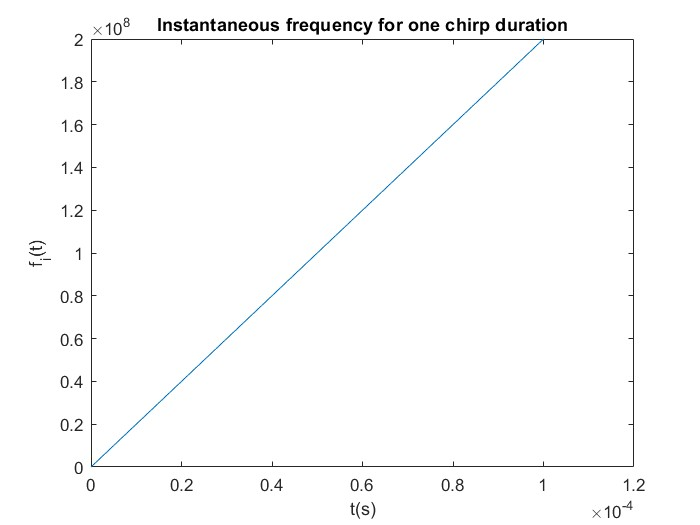
\includegraphics[scale = 0.25]{Pictures/one_chirp.jpg}
    \caption{\( f_i(t) \) pour un seul \textit{chirp} d'une durée de 0,4 ms }
    \label{fig:fi_t_chirp}
\end{figure}

Le signal transmis \( s(t) \) est modélisé par l'équation \ref{eq:s_transmis}.

\begin{equation} 
    s(t) = \cos(2\pi f_ct + \phi_i(t))
    \label{eq:s_transmis}
\end{equation}

où \( f_c \) est la fréquence porteuse et \( \phi_i(t) \) est la phase instantanée obtenue en intégrant \( f_i(t) \).

L'intégration de \( f_i(t) \) pour obtenir \( \phi_i(t) \) est formulée par l'équation \ref{eq:phi_inst}.

% Expression pour la phase instantanée
\begin{equation}
    \phi_i(t) = 2\pi \int_{0}^{t} f_i(u) \, du
    \label{eq:phi_inst}
\end{equation}

% Explication de l'intégrale
% Ici, \phi_i(t) représente la phase instantanée du signal FMCW, 
% calculée comme l'intégrale cumulée de la fréquence instantanée \( f_i(u) \) 
% sur l'intervalle [0, t]. Cela capture l'évolution de la phase du signal 
% en fonction du temps.

L'équation \ref{eq:signal_bb} permet la génération du signal en bande de base \( e^{j\phi_i(t)} \) 

\begin{equation}
    \text{signal en bande de base} = e^{(j \phi_i)}
    \label{eq:signal_bb}
\end{equation}

Ici, la fréquence instantanée \( f_i(t) \) est intégrée pour obtenir la phase instantanée \( \phi_i(t) \). Le signal en bande de base \( e^{j\phi_i(t)} \) est ainsi généré, représentant un \textit{chirp FMCW}.

En considérant le cas où le \textit{chirp} est répété indéfiniment sur le temps, similaire à un signal \textit{FMCW}, sa réponse en fréquence est échantillonnée à la cadence de répétition. Les conclusions tirées pour un seul \textit{chirp} dans cette étape sont donc généralisables à l'ensemble du signal \textit{FMCW}.

\section {Représentation du Signal en Temps et en Fréquence}

Cette génération de \textit{chirp} a été implantée en utilisant les paramètres suivants :
\begin{itemize}
  \item Plage de fréquence : \( B = 200 \, \text{MHz} \)
  \item Durée du \textit{chirp} : \( T = 0.2 \, \text{ms} \)
  \item Fréquence d'échantillonnage : \( F_s = 512 \, \text{MHz} \)
  \item Nombre d'échantillons : \( 2^{18} \)
\end{itemize}

%Le code Python associé permet de générer la fréquence instantanée \( f_i(t) \) en fonction du temps sur une durée de \textit{chirp}. Il permet aussi de produire le signal transmis en bande de base \( e^{j\phi_i(t)} \).

Les résultats ont été illustrés graphiquement, avec la partie réelle du signal en bande de base agrandie sur l'intervalle \( T \in [0; 4 \times 10^{-6}]\) dans la  sous-figure \ref{subfig:s_BB_zoom}, et la partie réelle du signal en bande de base sur l'intervalle \( T \in [0; 2T]\) dans la sous-figure \ref{subfig:s_BB_entier}.

\begin{figure}[H]
  \centering
  \begin{subfigure}[b]{0.45\textwidth}
    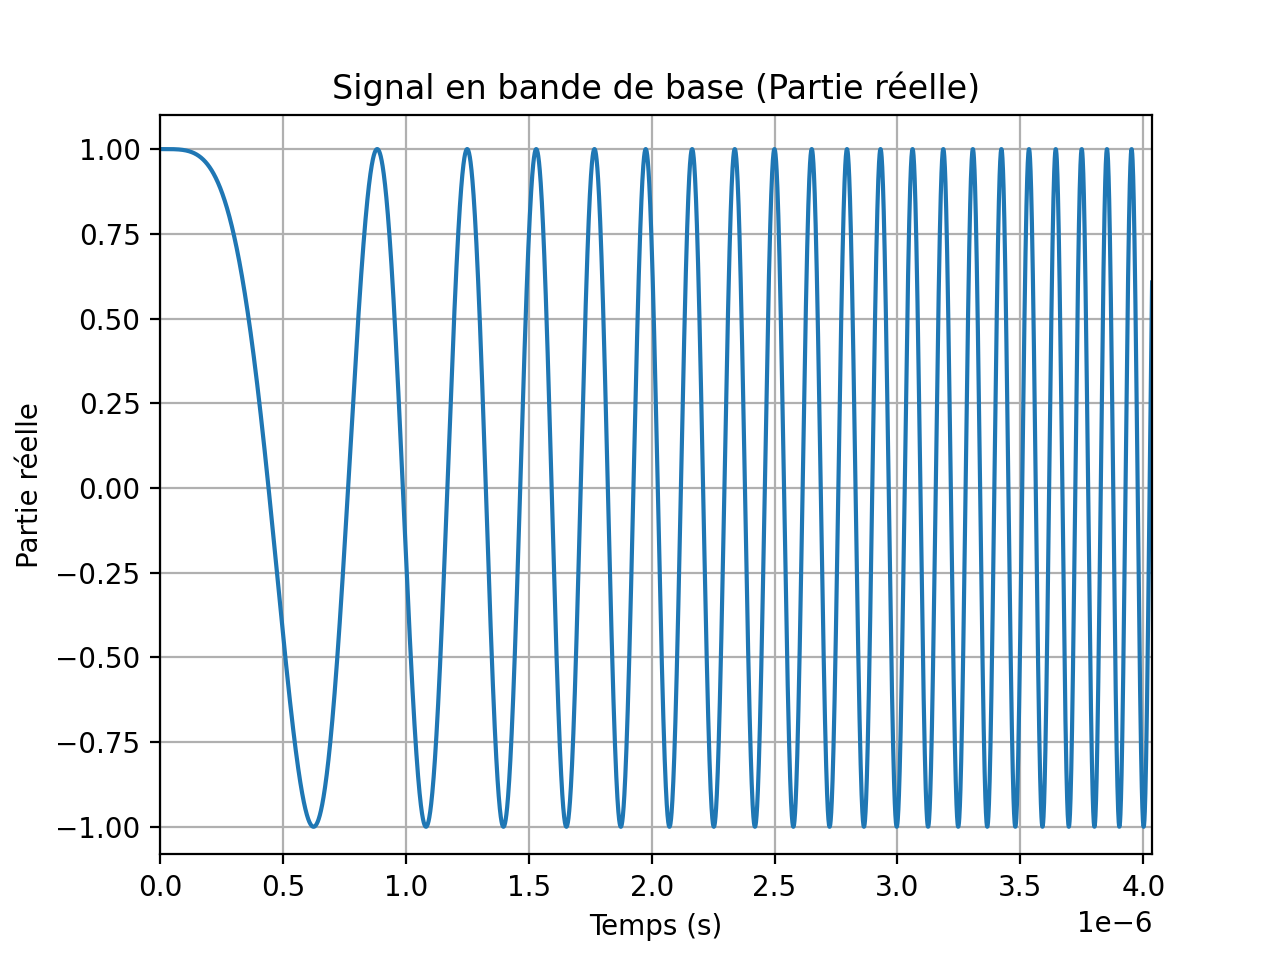
\includegraphics[width=\textwidth]{Pictures/BNDBR_SST.png}
    \caption{Partie réelle du signal en bande de base agrandie sur \(T \in [0; 4 \times 10^{-6}]\).}
    \label{subfig:s_BB_zoom}
  \end{subfigure}
  \hfill
  \begin{subfigure}[b]{0.45\textwidth}
    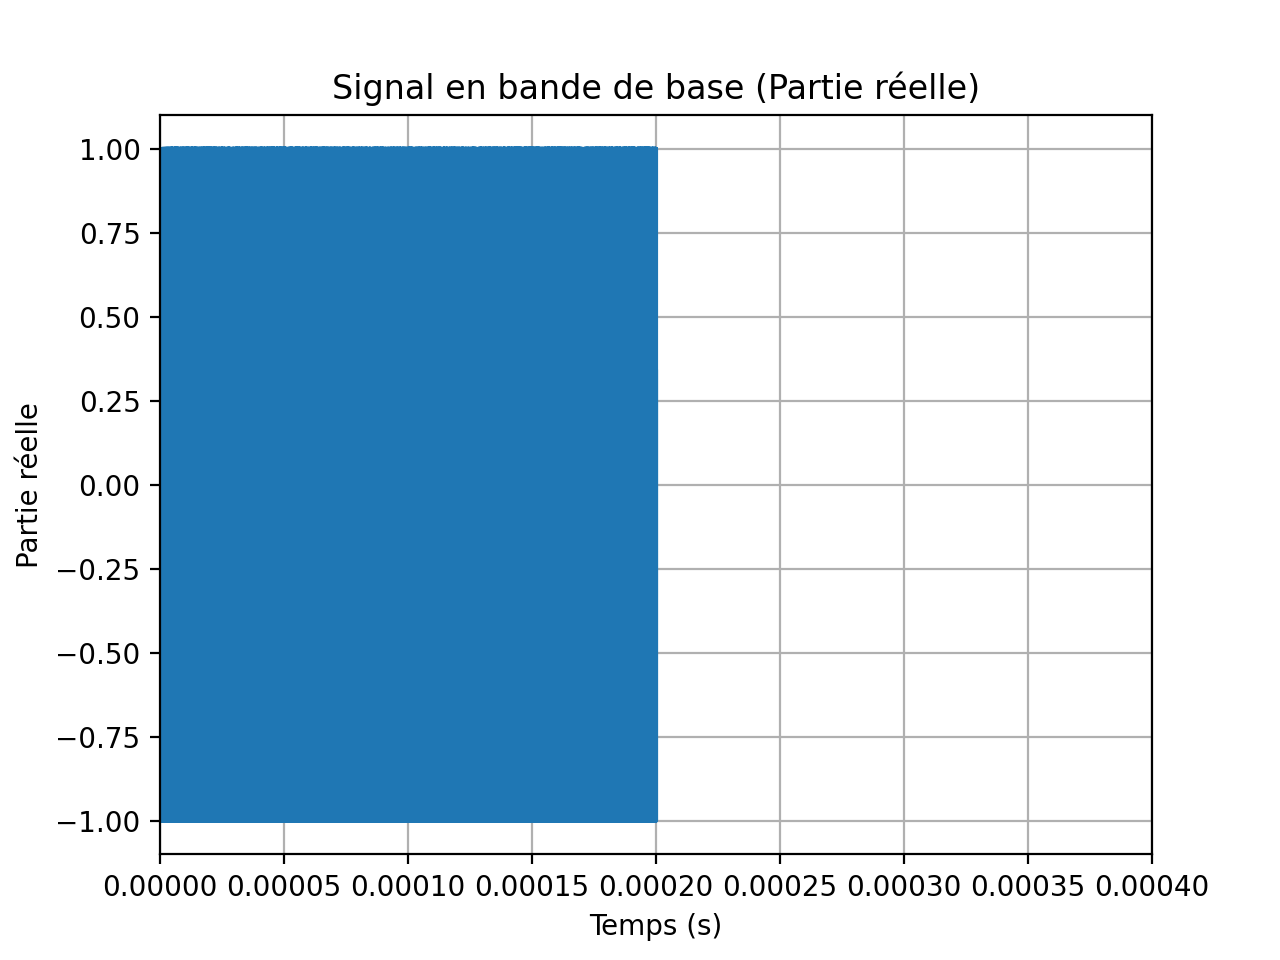
\includegraphics[width=\textwidth]{Pictures/BNDBR_SST(1).png}
    \caption{Partie réelle du signal en bande de base \(T \in [0; 2T]\).}
    \label{subfig:s_BB_entier}
  \end{subfigure}
  \caption{Représentation du \textit{chirp} dans le domaine temporel}
  \label{fig:chirp_temp}
\end{figure}

\section {Analyse Fréquentielle du Signal}

En effectuant la transformée de Fourier du signal, il est possible d'obtenir le spectre de fréquence en bande de base. La figure \ref{fig:spectre_bbs} représente l'amplitude du spectre de fréquence pour deux valeurs de $T$ différentes.

\begin{figure}[H]
  \centering
  \begin{subfigure}[b]{0.45\textwidth}
    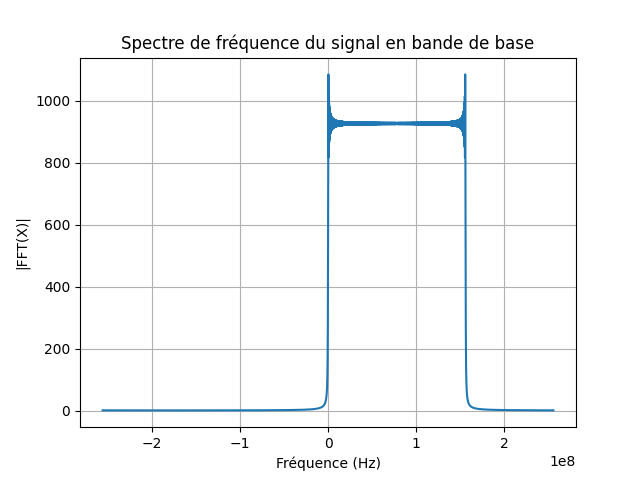
\includegraphics[width=\textwidth]{Pictures/SPCTR_SST.png}
    \caption{Spectre de fréquence du signal en bande de base pour $T=0.4$ms}
  \end{subfigure}
  \hfill
  \begin{subfigure}[b]{0.45\textwidth}
    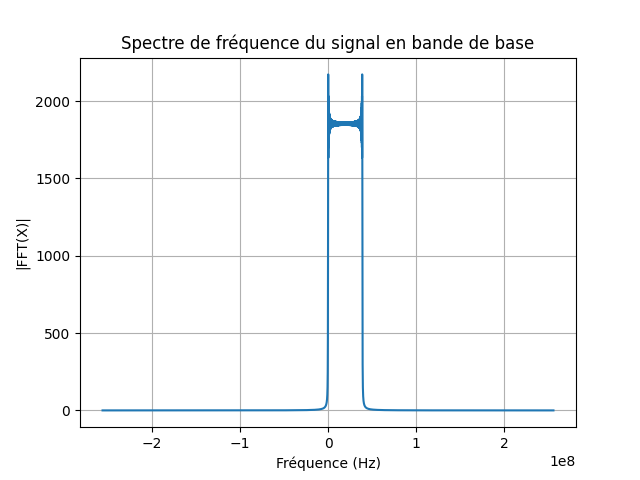
\includegraphics[width=\textwidth]{Pictures/SPCTR_SST(1).png}
    \caption{Spectre de fréquence du signal en bande de base pour $T=0.1$ms}
  \end{subfigure}
  \caption{Spectre de fréquence du signal en bande de base avec deux valeurs de $T$.}
  \label{fig:spectre_bbs}
\end{figure}

\section {Discussion de l'Impact de la Durée du \textit{Chirp} sur la Bande Passante}

Comme le montre la figure \ref{fig:spectre_bbs}, la durée du \textit{chirp} ($T$)  influence la plage de fréquences couvertes et donc la résolution en distance. Une durée plus longue permet une couverture fréquentielle plus étendue, améliorant la résolution en distance. Cependant, cela augmente également la consommation de bande passante, ce qui peut être limitant dans certaines applications.

